% -*- coding: UTF-8 -*-
% hurlex-chapt8.tex
% hurlex 开发文档 第8章内容

\section {完成中断请求和定时器中断}

\par 在上一章中我们完成了中断处理程序的框架,本章在其基础上讨论中断请求的实现。

\par 我们在上一章中提到,外设的所有中断由中断控制芯片8259A统一汇集之后连接到CPU的INTR引脚。\footnote{这里肯定会有读者提出来现代\allowbreak
的计算机主板上早就使用APIC(Advanced Programmable Interrupt Controller,高级可编程中断控制器)来进行外设的中断管理了。\allowbreak
没错,但是我相信在本科阶段的微机原理和接口技术中学的是8259APIC(Programmable Interrupt Controller),而且无论硬件怎么发展,\allowbreak
始终会兼容以前的接口。本着大家熟悉易理解的原则,我们依旧使用兼容的8259APIC(Programmable Interrupt Controller, 可编程中断控制器)\allowbreak
的设置方法进行设置。}这章我们就来探究8259APIC的初始化和实现定时器的中断处理。

\par 8259A PIC每一片可以管理8个中断源,显然一般情况下设备数量会超过这个值。这里就要提到IBM PC/AT 8259A PIC架构了,IBM的设计方案\allowbreak
是使用8259APIC的级联功能,使用两片级联(分为主、从片)的方式来管理硬件中断。其中主片的INT端连接到CPU的INTR引脚,从片的INT连接到\allowbreak
主片的IR2引脚。结构如下图所示:
\begin{figure}[ht]
      \centering
      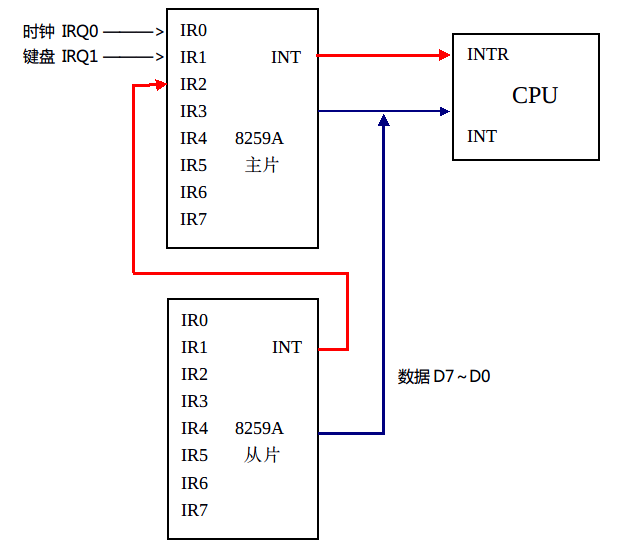
\includegraphics[scale=0.5]{picture/chapt8/8259A_PIC.png}
      \caption{8259A PIC级联}
\end{figure}

\par 图中时钟中断连接在主片的IRQ0引脚,键盘中断连接在了主片的IRQ1引脚。其它的引脚暂时用不到就不说了。在上一张描述中断描述符表时\allowbreak
我们知道了0~31号中断是CPU使用和保留的,用户可以使用的中断从32号开始。所以这里的IRQ0对应的中断号就是32号,IRQ1就是33号,然后以此\allowbreak
类推。

\par 理论就暂时阐述到这里,接下来是实现代码。首先是对8259A PIC的初始化,在设置中断描述符表的函数init\_idt最前面加入如下代码:

\begin{lstlisting}[language = C, caption = idt/idt.c]
// 初始化中断描述符表
void init_idt()
{	
	// 重新映射 IRQ 表
	// 两片级联的 Intel 8259A 芯片
	// 主片端口 0x20 0x21
	// 从片端口 0xA0 0xA1
	
	// 初始化主片、从片
	// 0001 0001
	outb(0x20, 0x11);
	outb(0xA0, 0x11);

	// 设置主片 IRQ 从 0x20(32) 号中断开始
	outb(0x21, 0x20);

	// 设置从片 IRQ 从 0x28(40) 号中断开始
	outb(0xA1, 0x28);
	
	// 设置主片 IR2 引脚连接从片
	outb(0x21, 0x04);

	// 告诉从片输出引脚和主片 IR2 号相连
	outb(0xA1, 0x02);
	
	// 设置主片和从片按照 8086 的方式工作
	outb(0x21, 0x01);
	outb(0xA1, 0x01);
	
	// 设置主从片允许中断
	outb(0x21, 0x0);
	outb(0xA1, 0x0);
	
	... ...
}
\end{lstlisting}

\par 对8259A PIC具体的设置我们不再阐述,这种资料网上铺天盖地的都是。相信结合注释很容易理解这个简单的初始化过程。

\par 完成了初始化之后,我们继续添加对IRQ处理函数的添加。首先是在idt.h头文件末尾添加如下内容:

\begin{lstlisting}[language = C, caption = include/idt.h]
// IRQ 处理函数
void irq_handler(pt_regs *regs);

// 定义IRQ
#define  IRQ0     32 	// 电脑系统计时器
#define  IRQ1     33 	// 键盘
#define  IRQ2     34 	// 与 IRQ9 相接,MPU-401 MD 使用
#define  IRQ3     35 	// 串口设备
#define  IRQ4     36 	// 串口设备
#define  IRQ5     37 	// 建议声卡使用
#define  IRQ6     38 	// 软驱传输控制使用
#define  IRQ7     39 	// 打印机传输控制使用
#define  IRQ8     40 	// 即时时钟
#define  IRQ9     41 	// 与 IRQ2 相接,可设定给其他硬件
#define  IRQ10    42 	// 建议网卡使用
#define  IRQ11    43 	// 建议 AGP 显卡使用
#define  IRQ12    44 	// 接 PS/2 鼠标,也可设定给其他硬件
#define  IRQ13    45 	// 协处理器使用
#define  IRQ14    46 	// IDE0 传输控制使用
#define  IRQ15    47 	// IDE1 传输控制使用

// 声明 IRQ 函数
// IRQ:中断请求(Interrupt Request)
void irq0();		// 电脑系统计时器
void irq1(); 		// 键盘
void irq2(); 		// 与 IRQ9 相接,MPU-401 MD 使用
void irq3(); 		// 串口设备
void irq4(); 		// 串口设备
void irq5(); 		// 建议声卡使用
void irq6(); 		// 软驱传输控制使用
void irq7(); 		// 打印机传输控制使用
void irq8(); 		// 即时时钟
void irq9(); 		// 与 IRQ2 相接,可设定给其他硬件
void irq10(); 		// 建议网卡使用
void irq11(); 		// 建议 AGP 显卡使用
void irq12(); 		// 接 PS/2 鼠标,也可设定给其他硬件
void irq13(); 		// 协处理器使用
void irq14(); 		// IDE0 传输控制使用
void irq15(); 		// IDE1 传输控制使用
\end{lstlisting}

\par 然后是idt\_s.s中添加相应的处理过程:

\begin{lstlisting}[language = {[x86masm]Assembler}, caption = gdt/gdt\_s.s]
; 构造中断请求的宏
%macro IRQ 2
[GLOBAL irq%1]
irq%1:
	cli
	push byte 0
	push byte %2
	jmp irq_common_stub
%endmacro

IRQ   0,    32 	; 电脑系统计时器
IRQ   1,    33 	; 键盘
IRQ   2,    34 	; 与 IRQ9 相接,MPU-401 MD 使用
IRQ   3,    35 	; 串口设备
IRQ   4,    36 	; 串口设备
IRQ   5,    37 	; 建议声卡使用
IRQ   6,    38 	; 软驱传输控制使用
IRQ   7,    39 	; 打印机传输控制使用
IRQ   8,    40 	; 即时时钟
IRQ   9,    41 	; 与 IRQ2 相接,可设定给其他硬件
IRQ  10,    42 	; 建议网卡使用
IRQ  11,    43 	; 建议 AGP 显卡使用
IRQ  12,    44 	; 接 PS/2 鼠标,也可设定给其他硬件
IRQ  13,    45 	; 协处理器使用
IRQ  14,    46 	; IDE0 传输控制使用
IRQ  15,    47 	; IDE1 传输控制使用

[GLOBAL irq_common_stub]
[EXTERN irq_handler]
irq_common_stub:
	pusha                    ; pushes edi, esi, ebp, esp, ebx, edx, ecx, eax
	
	mov ax, ds
	push eax                 ; 保存数据段描述符
	
	mov ax, 0x10  		 ; 加载内核数据段描述符
	mov ds, ax
	mov es, ax
	mov fs, ax
	mov gs, ax
	mov ss, ax
	
	push esp
	call irq_handler
	add esp, 4
	
	pop ebx                   ; 恢复原来的数据段描述符
	mov ds, bx
	mov es, bx
	mov fs, bx
	mov gs, bx
	mov ss, bx
	
	popa                     ; Pops edi,esi,ebp...
	add esp, 8     		 ; 清理压栈的 错误代码 和 ISR 编号
	iret          		 ; 出栈 CS, EIP, EFLAGS, SS, ESP
.end:
\end{lstlisting}

\par 最后是init\_idt函数构造IRQ的相关描述符和具体的IRQ处理函数了。

\begin{lstlisting}[language = C, caption = idt/idt.c]
// 初始化中断描述符表
void init_idt()
{	
	... ...
	idt_set_gate(31, (uint32_t)isr31, 0x08, 0x8E);

	idt_set_gate(32, (uint32_t)irq0, 0x08, 0x8E);
	idt_set_gate(33, (uint32_t)irq1, 0x08, 0x8E);
	idt_set_gate(34, (uint32_t)irq2, 0x08, 0x8E);
	idt_set_gate(35, (uint32_t)irq3, 0x08, 0x8E);
	idt_set_gate(36, (uint32_t)irq4, 0x08, 0x8E);
	idt_set_gate(37, (uint32_t)irq5, 0x08, 0x8E);
	idt_set_gate(38, (uint32_t)irq6, 0x08, 0x8E);
	idt_set_gate(39, (uint32_t)irq7, 0x08, 0x8E);
	idt_set_gate(40, (uint32_t)irq8, 0x08, 0x8E);
	idt_set_gate(41, (uint32_t)irq9, 0x08, 0x8E);
	idt_set_gate(42, (uint32_t)irq10, 0x08, 0x8E);
	idt_set_gate(43, (uint32_t)irq11, 0x08, 0x8E);
	idt_set_gate(44, (uint32_t)irq12, 0x08, 0x8E);
	idt_set_gate(45, (uint32_t)irq13, 0x08, 0x8E);
	idt_set_gate(46, (uint32_t)irq14, 0x08, 0x8E);
	idt_set_gate(47, (uint32_t)irq15, 0x08, 0x8E);

	// 255 将来用于实现系统调用
	idt_set_gate(255, (uint32_t)isr255, 0x08, 0x8E);

	... ...
}

// IRQ 处理函数
void irq_handler(pt_regs *regs)
{
	// 发送中断结束信号给 PICs
	// 按照我们的设置,从 32 号中断起为用户自定义中断
	// 因为单片的 Intel 8259A 芯片只能处理 8 级中断
	// 故大于等于 40 的中断号是由从片处理的
	if (regs->int_no >= 40) {
		// 发送重设信号给从片
		outb(0xA0, 0x20);
	}
	// 发送重设信号给主片
	outb(0x20, 0x20);

	if (interrupt_handlers[regs->int_no]) {
		interrupt_handlers[regs->int_no](regs);
	}
}
\end{lstlisting}

\par 结合代码中详细的注释和本章开始的8259A PIC的结构图,详细很容易理解这个处理过程。其实IRQ和ISR的处理过程很类似:
\begin{mdframed}
	\begin{itemize}
		\item ISR的处理过程是 (isr0 - isr31) -> isr\_common\_stub -> isr\_handler -> 具体的ISR处理函数。
		\item IRQ的处理过程是 (irq0 - irq15) -> irq\_common\_stub -> irq\_hanlder -> 具体的IRQ处理函数。
	\end{itemize}
\end{mdframed}

\par 写到这里具体的IRQ处理过程就完成了,以后只需要设置好相应的处理函数就好了,接下来我们实现时钟中断的产生和处理。

\par 时钟中断对于操作系统内核来说很重要的一种中断,它使得CPU无论在执行任何用户或者内核的程序时,都能定义的将执行权利\allowbreak
交还到CPU手中来。\footnote{当然了,屏蔽中断就没办法了。}除了记录时间之外,时钟中断的处理函数里通常都是对进程的调度处理。\allowbreak

\par 具体的时钟中断源是8253/8254 Timer 产成的,要按照需要的频率产生中断,需要先配置8253/8254 Timer芯片。代码如下:

\begin{lstlisting}[language = C, caption = drivers/timer.c]
#include "timer.h"
#include "debug.h"
#include "common.h"
#include "idt.h"

void timer_callback(pt_regs *regs)
{
	static uint32_t tick = 0;
	printk_color(rc_black, rc_red, "Tick: %d\n", tick++);
}

void init_timer(uint32_t frequency)
{
	// 注册时间相关的处理函数
	register_interrupt_handler(IRQ0, timer_callback);

	// Intel 8253/8254 PIT芯片 I/O端口地址范围是40h~43h
	// 输入频率为 1193180,frequency 即每秒中断次数
	uint32_t divisor = 1193180 / frequency;

	// D7 D6 D5 D4 D3 D2 D1 D0
	// 0  0  1  1  0  1  1  0
	// 即就是 36 H
	// 设置 8253/8254 芯片工作在模式 3 下
	outb(0x43, 0x36);

	// 拆分低字节和高字节
	uint8_t low = (uint8_t)(divisor & 0xFF);
	uint8_t hign = (uint8_t)((divisor >> 8) & 0xFF);
	
	// 分别写入低字节和高字节
	outb(0x40, low);
	outb(0x40, hign);
}
\end{lstlisting}

\par 对应的头文件如下:

\begin{lstlisting}[language = C, caption = include/timer.h]
#ifndef INCLUDE_TIMER_H_
#define INCLUDE_TIMER_H_

#include "types.h"

void init_timer(uint32_t frequency);

#endif 	// INCLUDE_TIMER_H_
\end{lstlisting}

\par 8253/8254 Timer有三种工作模式,我们使用第三种。init\_timer函数的参数是所需的时钟中断的频率,具体的设置原理不再赘述。\allowbreak
最后,修改入口函数进行测试:

\begin{lstlisting}[language = C, caption = init/entry.c]
#include "console.h"
#include "debug.h"
#include "gdt.h"
#include "idt.h"
#include "timer.h"

int kern_entry()
{
	init_debug();
	init_gdt();
	init_idt();

	console_clear();
	printk_color(rc_black, rc_green, "Hello, OS kernel!\n");

	init_timer(200);

	// 开启中断
	asm volatile ("sti");

	return 0;
}

\end{lstlisting}

\par 最后编译执行,我们看到了如下的输出:
\begin{figure}[ht]
      \centering
      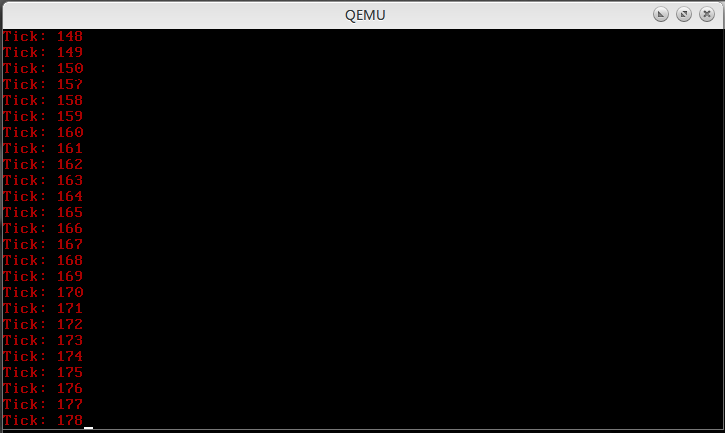
\includegraphics[scale=0.6]{picture/chapt8/8253_TIMER.png}
      \caption{8253/8254 Timer 中断}
\end{figure}

